% !TeX root = ../../../thesis.tex

\section{Simulation}
\label{sec:simulation-evaluation}

In \autoref{sec:hardware-evaluation} the evaluation of the hardware and software was shown using the continuous transmission method, as detailed in \autoref{subsec:continuous-method-modulation}.
Since this is already been evaluated and proven, in this simulation section the scalability of a larger system will be evaluated, using the probabilistic method as explained in \autoref{subsec:probabilistic-method-modulation}.


Before the actual simulation itself, parameters such as $\epsilon$ need to be set.
1 - $\epsilon$, is the probability that for every point in time the number of LEDs that are modulating will not exceed $m$, as discussed in \autoref{subsec:probabilistic-method-modulation}.
This will determine if interference can occur and therefor the overall accuracy and correctness of the system.

For the rest of this simulation a Gold sequence set with length 127 will be used for the assessment.

This simulation does the following: 

\begin{itemize}

	\item For the set values of the sequence set, $\epsilon$ and $\epsilon_1$, the probability $p$ and the number of runs $k$ are calculated (See \autoref{subsec:probabilistic-method-modulation}).

	\item For each run, from the total $k$ runs, it is decided which transmitters will transmit. The probability $p$ is used for this. $k$ depends on $p$ and $\epsilon_1$.

	\item If a certain transmitter is selected to transmit, its code sequence is added to a signal vector. One particular transmitter may be not selected at all, or many times, again probability $p$ is used for this.

	\item When the entire signal has been constructed, the decoding process begins. All sequences in the set are used to decode the incoming signal for every time step.

	\item During the decoding, the results are analyzed and together with the information that is known when a particular transmitter transmitted at what time, the results are classified into four categories: true-positive, true-negative, false-positive and false-negative. This is done per run.

	\item With those four categories, the precision, recall and the F-measure are calculated per run.



\end{itemize}




Let's set $\epsilon = 0.1$, meaning that the probability that there will be more than $m$ LEDs modulating for every point in time will be 0.9 or 90 \%.
Let's set $\epsilon_1 = \epsilon$, meaning the probability that all LEDs will have modulated at least once is equal to 0.9 or 90 \%.
With these values and the Gold sequence set with length 127, the simulation as described above can begin. 

The results of the simulation can be seen in \autoref{fig:sim-concurrent-tx-and-f-measure-eps=1-n=7}.
Also note that 17 \% of the transmitters did not transmit their sequence even once.
In the upper plot the number of concurrent transmitters can be seen. 
$m$ is also visible here.
When the number of concurrent transmitters is below the line $m$, it is guarantied that no interference will occur, as proven in \autoref{sec:interference-solution}.
But when the number of concurrent transmitters is above the line $m$, it is possible that there will be interference but it is not always the case.
This depends on what the cross correlation with the other sequences is and if they cancel each other out or if they enhance each other.
From the lower plot it can be seen that whenever the number of concurrent transmitters in the upper plot is below the $m$ line, the F-measure is equal to 1.
This means that everything in the decoding process went well, no false-positives and/or false-negatives.
When the number of concurrent transmitters is above the $m$ line, two things can happen: either there is enough interference to cause false-positives and/or false-negatives, or there is not enough interference and everything will go well.
Two times the number of concurrent transmitters is so high, it causes interference as can be seen in the F-measure, which has drops at the same run as when the number of concurrent transmitters are too high.

\begin{figure}[tbp]
	\centering
	\includegraphics[width=\textwidth]{chapters/evaluation-chapters/simulation/sim-concurrent-tx-and-f-measure-eps=1-n=7.eps}
	\caption{Results of the simulation. Upper plot shows the number of concurrent transmitters per run along with $m$. The lower plot shows the F-measure per run.}
	\label{fig:sim-concurrent-tx-and-f-measure-eps=1-n=7}
\end{figure}

17 \% of the transmitters did not transmit their sequence even once.
This is due to the relatively high value $\epsilon_1 = 0.1$.
There were $k = 84$ runs done.
This results in a time is equal to $\frac{127}{10000} \times 84 = 1.1$ s (See \autoref{eq:time-for-probabilistic-txs}).
So this was a very fast time and pretty accurate, considering that there were only two drops in the F-measure.
But a lot of transmitters did not even transmit once.










The same simulation is done again, but now with $\epsilon = \epsilon_1 = 0.001$.
The plots can be seen in \autoref{fig:sim-concurrent-tx-and-f-measure-eps=001-n=7}.
Note that all transmitters have transmitted at least once.
Only one time the number of concurrent transmitters goes above the $m$ line, but it does not cause interference as shown be the F-measure, which is a constant 1.
So with $\epsilon = \epsilon_1 = 0.001$ it is an accurate setup that can use all the sequences in the set.
But the number of runs is $k = 1023$.
This results in a time of $\frac{127}{10000} \times 1023 = 13.0$ s (See \autoref{eq:time-for-probabilistic-txs}).
This is still a relative small amount of time, but still 13 times larger than the previous simulation.


\begin{figure}[tbp]
	\centering
	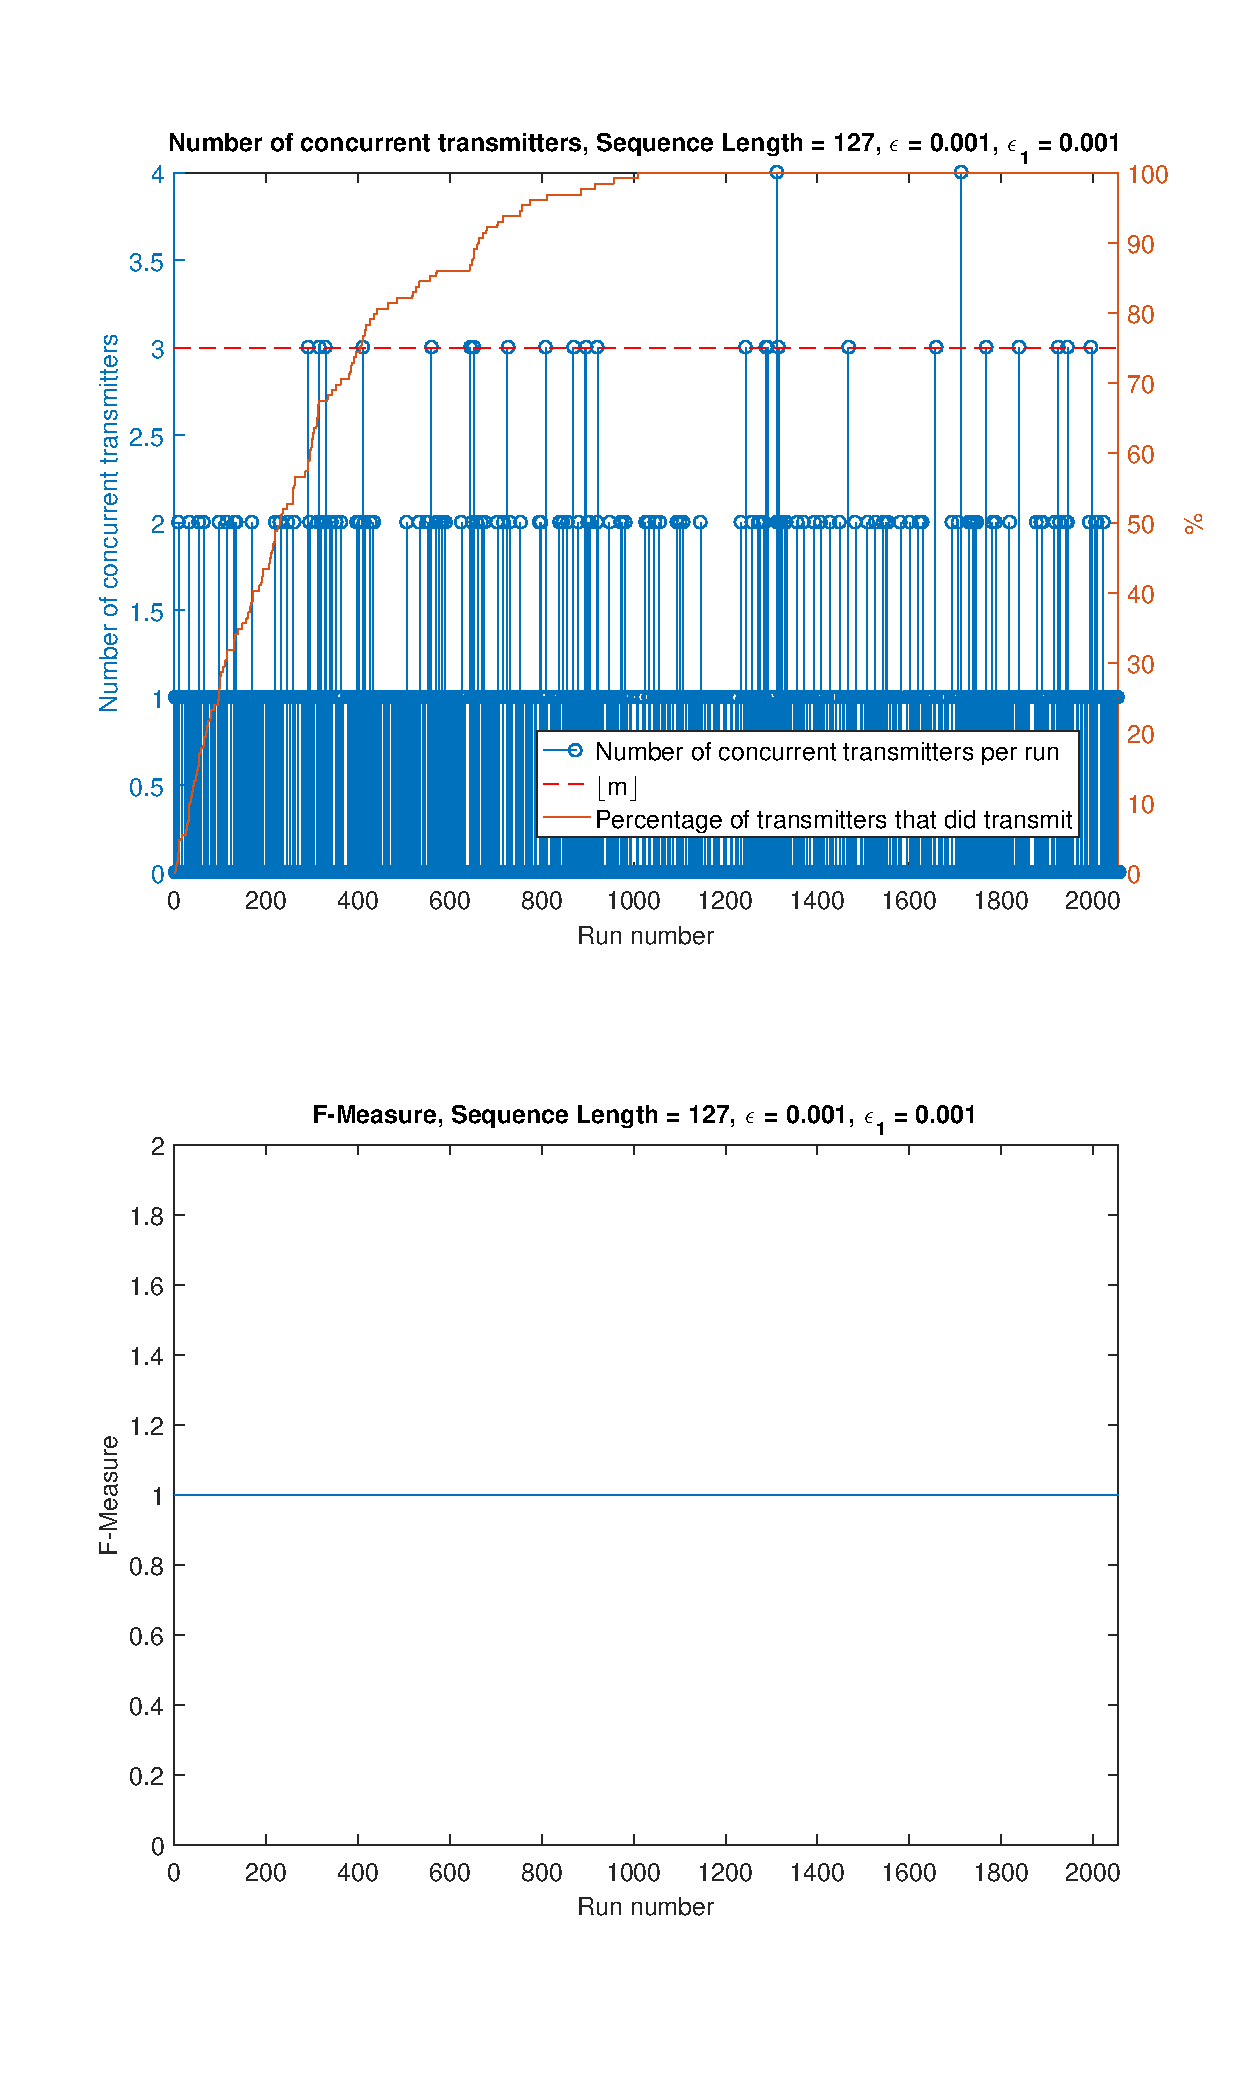
\includegraphics[width=\textwidth]{chapters/evaluation-chapters/simulation/sim-concurrent-tx-and-f-measure-eps=001-n=7.eps}
	\caption{Results of the simulation. Upper plot shows the number of concurrent transmitters per run along with $m$. The lower plot shows the F-measure per run.}
	\label{fig:sim-concurrent-tx-and-f-measure-eps=001-n=7}
\end{figure}

 

These simulations show that for the probabilistic method there is a clear trade off between time and accuracy.